% !TeX root = ../main.tex

\newcommand{\researchq}[1]{%
  \textbf{RQ~#1}\label{rq:#1}%
}

\newcommand{\rqref}[1]{%
  \hyperref[rq:#1]{RQ\textsubscript{#1}}%
}

\newcommand{\Mdn}{\mathrm{Mdn}}
\newcommand{\dMdn}{\Delta\mathrm{Mdn}}
\DeclareSIUnit{\pp}{pp}

\chapter{Evaluation}\label{chapter:evaluation}
This chapter evaluates the approach presented in \autoref{chapter:approach} in two studies.
The first examines how the pipeline should be configured by varying the starting corpus and the scope of the \ac{CoI}, and measuring the effectiveness of the resulting seed corpora.
The second takes the configuration selected there and evaluates it end-to-end, comparing the augmented corpus against the project's original corpus in fuzzing campaigns targeting known regression bugs.
\num{6} subjects are used to select the configuration; the fuzzing study adds another \num{6} held-out subjects, so that the end-to-end results can be read separately for projects that did and did not inform that choice.
\autoref{sec:eval:setup} describes the subjects and the shared experimental infrastructure, \autoref{sec:eval:statistics} the statistical procedures employed, \autoref{sec:eval:seedgen} and \autoref{sec:eval:fuzzing} report the two studies, and \autoref{sec:eval:threats} discusses threats to validity.

\section{Experimental Setup}\label{sec:eval:setup}
\subsection{Subjects}\label{sec:eval:subjects}
\begin{table*}
\centering
\footnotesize
\setlength{\tabcolsep}{4pt}
\begin{tabular}{l p{2.4cm} r l r r r S[table-format=2.1] r S[table-format=2.1]}
\toprule
 &  &  &  &  &  & \multicolumn{2}{c}{Affected} & \multicolumn{2}{c}{Overall} \\
\cmidrule(lr){7-8}\cmidrule(lr){9-10}
Name & Project & \makecell[r]{Size\\(LoC)} & \makecell[l]{Failure\\type} & Seeds & \makecell[r]{Chg.\\lines} & Lines & {Cov.\%} & Lines & {Cov.\%} \\
\midrule
\texttt{curl-8000}          & Network data transfer     & 184K & Buf-overrun    & 4,202  & 51  & 16,379 & 47.0 & 40,416  & 44.7 \\
\texttt{harfbuzz-55779}     & Text-to-font rendering    & 135K & Assert violat. & 1,003  & 105 & 13,387 & 61.9 & 43,729  & 41.6 \\
\texttt{libhtp-17198}       & HTTP protocol parser      & 40K  & Buf-overrun    & 97     & 26  & 3,656  & 64.4 & 8,910   & 56.0 \\
\texttt{libxml2-17737}      & XML parsing               & ---  & Use-aft-free   & 1,309  & 32  & 37,427 & 9.4  & 98,005  & 6.6  \\
\texttt{ndpi-49057}         & Deep packet inspector     & 93K  & Int-overflow   & 351    & 51  & 12,045 & 2.7  & 35,397  & 15.1 \\
\texttt{openssl-17715}      & SSL/TLS cryptography      & 592K & Buf-overrun    & 2,240  & 91  & 47,152 & 15.0 & 116,691 & 13.9 \\
\texttt{pcap++-23592}       & Packet processing         & 59K  & Buf-overrun    & 615    & 32  & 1,901  & 27.1 & 13,119  & 17.0 \\
\texttt{poppler-35789}      & PDF file rendering        & 198K & Null-deref     & 476    & 3   & 31,086 & 6.9  & 96,010  & 5.5  \\
\texttt{readstat-13262}     & Statistics data converter & 31K  & Buf-overrun    & 94     & 5   & 521    & 58.0 & 2,478   & 36.4 \\
\texttt{usrsctp-18080}      & SCTP protocol             & 85K  & Use-aft-free   & 156    & 6   & 10,090 & 19.9 & 50,277  & 18.1 \\
\texttt{yara-38952}         & Malware detector          & 63K  & Buf-overrun    & 9      & 277 & 7,644  & 20.7 & 28,119  & 18.5 \\
\texttt{zstd-21970}         & Data compression          & 104K & Null-deref     & 12,462 & 280 & 6,124  & 69.5 & 30,600  & 34.3 \\
\bottomrule
\end{tabular}
\caption{Benchmark subjects and starting-corpus coverage.}
\label{tab:subjects}
\end{table*}

The subjects are drawn from the BugOSS benchmark by Kim and Hong~\cite{kimBugOssBenchmarkRealworld2024}, a collection of reproducible real-world regression bugs in OSS-Fuzz projects.
For each bug, it provides the \ac{BIC}, the bug-fixing commit, a bug-revealing input, the locations of the bug and of the fix, and scripts to build the respective project.
The \ac{BIC} is what makes the benchmark suitable here, as it defines the change from which the \ac{CoI} is computed.
BugOSS is also the benchmark used by the prior work from which the \ac{CoI} computation is taken, which keeps the cost of reusing that tooling low.
In the remainder of this chapter, a project such as libhtp refers to that project at its \ac{BIC}, where the respective bug has just been introduced.

Of the \num{21} projects in BugOSS, \num{9} were excluded.
\num{5} fail a precondition of the setup.
\emph{arrow} is excluded because its defect is not related to memory access and thus falls outside the addressed bug class, for which the metrics presuppose a sanitizer-detectable memory error at a crash site.
\emph{grok} is excluded because its \ac{BIC} is no longer available on GitHub, so no \ac{CoI} can be derived.
\emph{gdal} is excluded because its bitcode is too large for the static analysis, which terminates out of memory.
\emph{aspell} and \emph{file} are excluded because their harnesses read configuration files supplied outside the seed corpus; as the \ac{LLM} never observes these files, the augmentation arms would be handicapped by an artifact of the harness rather than by the property under study.
\emph{openh264} is excluded because its \ac{BIC} consists solely of removals.
The underlying \ac{CoI} computation takes the lines Git classifies as added in the \ac{BIC} as its slicing criterion, and this set is empty for this project.
Admitting it would require deviating from the procedure applied to every other subject.
The remaining three exclusions, \emph{libarchive}, \emph{exiv2}, and \emph{leptonica}, were made to keep the evaluation within budget; these were not excluded based on a systematic criterion.
This leaves \num{12} subjects, \num{6} of which are also used to select the configuration in \autoref{sec:eval:seedgen}; the split is carried through every table and plot in \autoref{sec:eval:fuzzing}.



\subsection{Infrastructure and Configuration}
All experiments were carried out on a single Fujitsu CELSIUS M770 workstation running Ubuntu 24.04.4 LTS (kernel 6.8.0).
The machine is equipped with a \num{6}-core Intel Xeon W-2133 (Skylake, \num{12} hardware threads, \SIrange{1.2}{3.9}{\giga\hertz}, \SI{8.25}{\mebi\byte} L3), \SI{64}{\gibi\byte} of RAM, and an NVMe SSD holding all target builds and corpora.
Targets are not built on the host: each subject is compiled inside its OSS-Fuzz build container, so the toolchain, sanitizer configuration, and harness definitions are those the project uses upstream and vary between subjects.
Fuzzing campaigns are likewise executed in OSS-Fuzz runner containers, each campaign pinned to a dedicated hardware thread.
All campaigns use AFL++~5.03a (stable).

Seed generation uses DeepSeek-V4-Flash-0731~\cite{deepseek-aiDeepSeekV4HighlyEfficient2026}, a \num{304}-billion-parameter MoE model released under the MIT license, accessed through the provider's hosted \ac{API} rather than served locally.
The model was selected as the strongest openly licensed model with agentic capabilities available at the lowest cost per token at the time of the experiments.
All requests were issued during August~2026 against the \texttt{deepseek-v4-flash} endpoint; since hosted endpoints may be updated without notice, the results reported here are tied to that period.
Following the model's recommended settings for agentic use, sampling uses a temperature of \num{1.0} and $\text{top-}p$ of \num{0.95}, at the \texttt{high} reasoning effort level.

To constrain the cost of the generation process, the agent is subject to a \num{20}-cycle limit (i.e., \num{20} opportunities to generate seed inputs and receive feedback) and a soft-to-hard budget range of \SIrange{0.45}{0.50}{\USD} for the fuzzing study and \SIrange{0.30}{0.35}{\USD} for the more extensive generation study.
Across all experiments, this resulted in a total expenditure of around \SI{50}{\USD}.
The \num{20}-cycle limit was established during prototyping and represents a pragmatic balance: it affords the LLM agent sufficient opportunities to iteratively generate, test, and refine candidate seeds, while mitigating excessive expenditure and limiting the risk of diminishing returns from prolonged generation.

\section{Statistical Procedure}\label{sec:eval:statistics}

Raw measurements are not directly comparable across projects because their numerical scales and attainable values can differ substantially.
The analysis therefore proceeds in two stages: configurations are compared within each project, where they share the same target, and the resulting project-level outcomes are aggregated across projects using ranks and normalized scores.
This follows established practice for cross-benchmark evaluation in fuzzing and software engineering \cite{demsar2006,metzman2021,klees2018,arcuri2014,schloegelSoKPrudentEvaluation2024}.
Table~\ref{tab:statistical-procedure} summarizes the statistical tests and magnitude measures used in each stage.

\paragraph{Effect and significance.}
For each comparison, statistical significance, effect size, and practical measure are considered separately.
Statistical tests assess whether the observed difference provides sufficient evidence against the null hypothesis.
The null hypothesis assumes that the compared configurations do not exhibit a systematic difference in the respective outcome.
A $p$-value below $\alpha=\num{0.05}$ is therefore interpreted as evidence against this hypothesis.
Effect sizes quantify the magnitude and direction of an observed difference independently of the original measurement scale, whereas practical measures express the difference in the original units of the metric, such as coverage, time, or corpus size.
Thus, statistical significance indicates evidence for a difference, while effect size and practical measure indicate its magnitude and practical relevance.

The attainable significance level is constrained by the small number of campaigns and projects; consequently, even complete separation of the observed outcomes may not yield $p<\num{0.05}$.
A non-significant result is therefore not interpreted as evidence of equivalence.
Effect estimates and confidence intervals are reported regardless of significance to convey the observed direction and magnitude of the differences.

\paragraph{Within-project comparisons.}
The first stage evaluates configurations within each project.
Each arm corresponds to one configuration, and repeated campaigns with different random seeds provide the observations.

For two arms, the Mann--Whitney $U$ test \cite{mann1947} is used for continuous outcomes, as it asks whether draws from one arm tend to exceed draws from the other without assuming normality or equal variances.
The Vargha--Delaney $\hat{A}_{12}$ measure \cite{vargha2000} quantifies the effect size, giving the probability that a randomly chosen run of one arm outperforms a randomly chosen run of the other, while the difference in medians represents the practical measure in the original metric.
For binary outcomes, Fisher's exact test \cite{fisher1922} is used because it directly evaluates differences in success rates and, being exact rather than asymptotic, remains appropriate for the small sample sizes considered here.
The difference in success rates is reported as the practical measure.

For three arms, the Kruskal--Wallis test \cite{kruskal1952} is first used as an \emph{omnibus} test for continuous outcomes, extending the same rank comparison from two samples to three.
The omnibus test indicates, if significant, that the three arms do not stem from the same distribution, but does not indicate which arm differs from the others.
A \emph{post-hoc} test is therefore needed, and Dunn's test \cite{dunn1964} provides the three pairwise comparisons by contrasting the arms' mean ranks from the omnibus' joint ranking, so that gate and post hoc cannot reach contradictory conclusions.
The Holm correction \cite{holm1979} is applied to the resulting $p$-values because it controls the family-wise error rate across the three comparisons.
Effect size and practical measure are reported per comparison as above.
Binary outcomes are not compared across three configurations.

\paragraph{Across-project aggregation.}
The second stage treats projects as matched units, since each configuration is evaluated on the same set of projects.
Each project, therefore, contributes one project-level summary value per configuration.
Before aggregation, metrics are oriented such that larger values consistently indicate better performance.

For two configurations with continuous outcomes, the paired project-level summaries are compared using the Wilcoxon signed-rank test \cite{wilcoxon1945}.
The Hodges--Lehmann estimator $\hat{\Delta}_{\mathrm{HL}}$ \cite{hodges1963} provides a robust estimate of the paired shift between configurations and, because it is expressed in the original metric units, serves as the practical effect measure.
For binary outcomes, the paired success outcomes across projects are compared using the sign test \cite{dixon1946}.
Unlike the Wilcoxon test, the sign test considers only the direction of the paired differences and therefore does not rely on their magnitude or distribution.
The difference in success rates across projects is reported as the practical effect.

For three configurations with continuous outcomes, the Friedman test \cite{friedman1937} is used as an omnibus test for the matched project blocks.
Two complementary scoring measures are then used: the within-project rank, where rank~1 denotes the best configuration, and a normalized score relative to the best configuration, which receives a score of~\num{100}.
Their averages across projects provide measures of consistency and relative performance, respectively, that are better than a pure rank~\cite {metzman2021}.
Significant results are followed by Nemenyi \emph{post-hoc} pairwise comparisons \cite{nemenyi1963} to isolate the pairs that differ.

\begin{table}[t]
  \centering
  \begin{threeparttable}
    \footnotesize
    \setlength{\tabcolsep}{3pt}
    \begin{tabular*}{\textwidth}{@{\extracolsep{\fill}}lll@{}}
      \textbf{Comparison} & \textbf{Significance test} & \textbf{Magnitude measure} \\
      \midrule
      \addlinespace[2pt]
      \multicolumn{3}{@{}l}{\textsc{Within-project}\ \textnormal{(campaigns of one subject)}} \\
      \addlinespace[1pt]
      \hspace{1em}2 arms, continuous & Mann--Whitney $U$ \cite{mann1947} & $\hat{A}_{12}$ \cite{vargha2000}; median difference \\
      \hspace{1em}2 arms, binary & Fisher's exact \cite{fisher1922} & Success-rate difference \\
      \hspace{1em}3 arms, continuous & Kruskal--Wallis \cite{kruskal1952} $\rightarrow$ Dunn \cite{dunn1964} & -- \\
      \addlinespace[6pt]
      \multicolumn{3}{@{}l}{\textsc{Across-project}\ \textnormal{(one paired value per subject)}} \\
      \addlinespace[1pt]
      \hspace{1em}2 arms, continuous & Wilcoxon signed-rank \cite{wilcoxon1945} & Hodges--Lehmann $\hat{\Delta}_{\mathrm{HL}}$ \cite{hodges1963} \\
      \hspace{1em}2 arms, binary & Sign test \cite{dixon1946} & Success-rate difference \\
      \hspace{1em}3 arms, continuous & Friedman \cite{friedman1937} $\rightarrow$ Nemenyi \cite{nemenyi1963} & Mean rank; normalized score~\cite{kimBugOssBenchmarkRealworld2024} \\
      \bottomrule
    \end{tabular*}
    \caption{Overview of the statistical tests and magnitude measures used in the evaluation.}
    \label{tab:statistical-procedure}
  \end{threeparttable}
\end{table}


\section{Pipeline Configuration Study}\label{sec:eval:seedgen}
To determine how the pipeline should be configured for regression fuzzing, the following research questions are addressed:

\begin{description}
  \item[\researchq{1.1} (starting corpus)] Which starting corpus yields the most effective seed corpus?
  \item[\researchq{1.2} (\ac{CoI} scope)] Which \ac{CoI} scope yields the most effective seed corpus?
\end{description}

For \rqref{1.1}, three starting corpora are compared: \emph{empty} (E), where no initial seeds are provided; \emph{distilled} (D), where the original corpus is reduced to a minimal set of seeds covering the affected code; and \emph{original} (O), where the complete initial corpus is provided.
For \rqref{1.2}, a \emph{full} \ac{CoI} scope is compared with a \emph{bounded} one, which restricts the code context given to the LLM to the changed code and its immediate surroundings, rather than all code reachable from the change.

Only one factor is varied at a time.
\rqref{1.1} is answered at a fixed \ac{CoI} scope.
\rqref{1.2} is then answered at the starting corpus selected by \rqref{1.1}, so the recommended combination is measured directly rather than inferred.
This ordering keeps the study within budget.
The cost is that the effect of \ac{CoI} scope is characterized only for the selected starting corpus.
Taken together, the two research questions identify the starting corpus and \ac{CoI} scope that yield the most useful seed corpus, within this restriction.

\subsection{Subjects}\label{sec:eval:seedgen:subjects}
This study uses \num{6} of the \num{12} subjects.
Two considerations motivate the restriction.
First, this is the study in which the configuration is selected, so every subject used informs the result.
Confining it to a subset leaves \num{6} projects that played no part in that choice, allowing the campaigns in \autoref{sec:eval:fuzzing} to be read separately for subjects that did and did not influence it.
Second, the cost per subject is asymmetric: this study runs \num{4} arms with \num{5} repetitions each, whereas the fuzzing study constructs each corpus once and varies only the campaigns.
The metered token budget is therefore consumed almost entirely here.

Within these constraints, the subset was chosen to span the dimensions along which seed generation is expected to vary.
The primary stratification is input format, since an \ac{LLM}'s ability to synthesize valid inputs plausibly depends on whether the format exposes human-readable structure; the subset is balanced evenly between mixed text-binary formats and purely binary ones.
It further covers \num{3} classes of memory-safety defect, program sizes spanning an order of magnitude, and both seed-scarce and seed-rich starting conditions.
These \num{6} subjects recur in \autoref{sec:eval:fuzzing} as the \emph{tuning subjects}.

\subsection{Procedure}\label{sec:eval:seedgen:procedure}
Each of the \num{6} subjects is augmented \num{5} times per configuration, starting from identical conditions, to account for the non-determinism of the underlying model.
\num{5} repetitions constitute the upper limit: this number still supports inference while staying within the research budget.
Trials are bounded by both a cycle and a cost budget (\cref{sec:eval:setup}) and are terminated on either one; the implications are discussed in \cref{sec:eval:threats}, and the termination condition for each project is itemized in \cref{tab:termination-campaigns}.

\paragraph{Metrics.}
The primary metric is \acf{CACC}, the percentage of lines covered by the whole corpus within the forward static slice taken from the commit change site (\cref{chapter:background}); higher is better.
It is what the agent augments against and, per \cref{sec:eval:fuzzing}, predicts the head start handed to the fuzzer.
The secondary metric is corpus size in seeds, lower being better, as a bloated corpus inflates the fuzzer's search space and I/O time.

For \rqref{1.2}, the volume of commit-affected code is bounded with the tool's distance-limiting policy, under which only slices within \num{10} basic blocks of the change site in the \ac{SVF} count as affected.
Arm~A uses this bounded cone ($\mathrm{CoI}_{10}$), arm~B the full cone ($\mathrm{CoI}_{\infty}$).
The scope is a single pipeline parameter that governs both the region reported to the agent as its coverage target and the selection of starting points, so the comparison measures the combined effect of the parameter rather than isolating either stage.
The starting corpus is fixed to the configuration selected in \rqref{1.1}.
The target-size reduction achieved by bounding the cone is quantified first, and the resulting safety implications are assessed by measuring the inclusion of regression crash sites.
Afterward, both arms are measured on the coverage of the two disjoint regions: the bounded cone ($\mathrm{CACC}_{10}$) and its complement, the part of the full cone beyond distance~\num{10} ($\mathrm{CACC}_{\infty \setminus 10}$).

\paragraph{Decision Rule.}
For \rqref{1.1}, criteria are applied in order: affected-code coverage, then corpus size.
An arm is selected at a criterion only if it significantly outperforms both others; otherwise, selection passes to the next criterion, and finally to the normalized score.

For \rqref{1.2}, the full scope is the default.
Bounding is selected only if it preserves reachability and covers significantly more of the bounded region than the full configuration does; coverage of the complement is reported as the cost of that choice.

\subsection{Results}
The results for \rqref{1.1} and \rqref{1.2} are presented in turn, following the order in which the pipeline is configured: the starting-corpus configuration is selected first, then fixed for the \ac{CoI}-scope comparison.
Each question is resolved by applying the decision rule from \cref{sec:eval:seedgen:procedure}.

\begin{tcolorbox}[colback=black!4, colframe=black!40, boxrule=0.4pt, left=6pt, right=6pt, top=6pt, bottom=6pt]
\paragraph{{\textbf{\rqref{1.1}}}}
The pipeline should be configured with the \emph{distilled} starting corpus: it leads on the normalized coverage score (\num{98}) at a near-best corpus size score (\num{88}), but since neither criterion produced an arm that significantly outperformed both others, this is a preference under a tie rather than an established difference.
\end{tcolorbox}

\begin{figure}
    \centering
    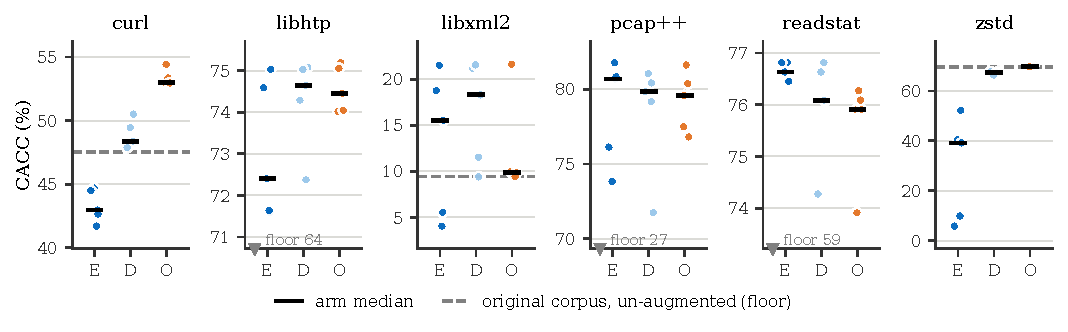
\includegraphics[width=\textwidth]{figures/rq1/corpus_coverage.pdf}
    \caption{\ac{CACC} of the final corpus across starting-corpus configurations}
    \label{fig:rq1:corpus_coverage}
\end{figure}

\paragraph{Affected-Code Coverage.}
The \ac{CACC} of the final corpus after the pipeline has run is depicted for each project under each starting-corpus configuration in \cref{fig:rq1:corpus_coverage}.
Across projects and arms, the median corpus improves on the un-augmented baseline, confirming that the agent contributes coverage of the affected code rather than merely preserving what the original corpus already reaches.
The exception is the \emph{empty} configuration, in which the agent must construct the entire corpus from scratch: on \texttt{curl} (\SI{-4.6}{\pp}) and \texttt{zstd} (\SI{-30.5}{\pp}) it does not recover the coverage that the original corpus provides for free.
The magnitude on \texttt{zstd} is the largest shortfall observed anywhere in the study, and it is accompanied by the widest within-arm spread, indicating that synthesizing valid inputs for this subject from nothing is both costly and unreliable.
Gains on \texttt{zstd} are slight in the other arms as well: starting from the \emph{original} corpus the agent adds only \SI[explicit-sign]{+0.3}{\pp}, and starting from the \emph{distilled} corpus it fails to recover what distillation discarded, ending \SI[explicit-sign]{-2.3}{\pp} below the baseline.
Distillation is therefore not uniformly reversible: reducing the corpus to a minimal covering set can remove structure that the agent cannot reconstruct within the trial budget.

The converse also holds, and more consistently: a complete starting corpus is not an advantage everywhere, and on \num{3} of the \num{6} subjects it is a liability.
On \texttt{readstat} and \texttt{pcap++} the \emph{empty} arm attains the highest median, marginally ahead of both other configurations, so the entire contribution of the supplied seeds is matched by an agent starting from nothing.
\texttt{libxml2} is the pronounced case: the \emph{original} arm finishes at a median of \SI{10.0}{\percent}, barely clearing the baseline of \SI{9.5}{\percent}, while \emph{distilled} reaches \SI{18.2}{\percent} and even \emph{empty} reaches \SI{15.5}{\percent} from no seeds at all.
Handing the agent the full corpus here leaves it close to where it started, whereas removing all but the seeds that touch the affected code nearly doubles the final coverage.
The pattern suggests that a large corpus occupies the agent's context with seeds that are irrelevant to the change site and anchors its synthesis to what those seeds already exercise, an effect that the distilled configuration avoids by construction and that the empty configuration cannot suffer from at all.

These per-project differences do not add up to a separation between arms.
The per-project tests in the \ac{CACC} block of \cref{tab:seeding-dimensions}, where arms are reported as scores normalized per project, resolve a pair on only two subjects, \texttt{curl} and \texttt{zstd}, in both cases \emph{original} over \emph{empty}; the remaining four yield no significant pair, with \texttt{libxml2} and \texttt{pcap++} at $p_{Holm} = \num{1.000}$ despite the spread visible in \cref{fig:rq1:corpus_coverage}.
Across all \num{6} projects the arms are indistinguishable ($p_{Holm} = \num{0.740}$), with \emph{empty} and \emph{original} tied at mean rank \num{2.17} and \emph{distilled} only slightly ahead at \num{1.67}.
No arm significantly outperforms both others on this criterion, so by the decision rule of \cref{sec:eval:seedgen:procedure} selection passes to corpus size.

\paragraph{Corpus Size and Composition.}
The composition of the final corpus is depicted in \cref{fig:rq1:corpus_size}, separating the seeds inherited from the starting corpus from those the agent generated during augmentation.
The generated component is strikingly insensitive to the configuration it starts from: on every subject and in every arm, it falls between roughly \numrange{100}{1000} seeds, and within a subject, the three arms generate counts of the same order.
The agent, therefore, produces an almost fixed volume of output per trial, governed by the cycle and cost budget rather than by what it was given, and the differences in final corpus size between arms are almost entirely inherited rather than earned.

\begin{figure}
    \centering
    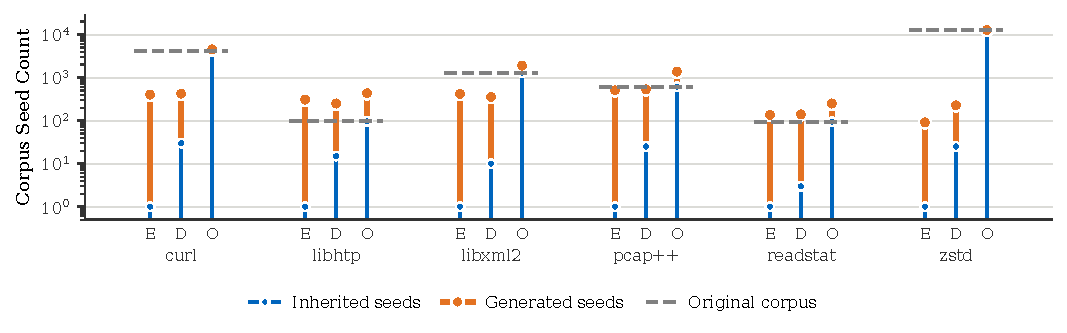
\includegraphics[width=\textwidth]{figures/rq1/corpus_size.pdf}
    \caption{Seed count of the final corpus across starting-corpus configurations}
    \label{fig:rq1:corpus_size}
\end{figure}

What separates the arms is consequently how much of the original corpus survives into the final one.
Distillation reduces the starting corpus by one to three orders of magnitude, most sharply on the seed-rich subjects: \texttt{zstd} falls from roughly \num{12000} seeds to \num{25}, \texttt{curl} from \num{4000} to \num{28}, and \texttt{libxml2} from \num{1300} to \num{10}.
Because the generated component is of fixed order, the \emph{distilled} arm ends within the same order of magnitude as \emph{empty} on every subject, whereas \emph{original} carries its full corpus through and ends an order of magnitude or more above both.
The extreme is \texttt{zstd}, where the \emph{original} arm finishes at roughly \num{12000} seeds against \num{230} for \emph{distilled}.

Read against \cref{fig:rq1:corpus_coverage}, this is where the \emph{original} configuration is least defensible.
On \texttt{zstd} its \num{12000} seeds buy \SI[explicit-sign]{+0.3}{\pp} over the un-augmented baseline, and on \texttt{libxml2} its \num{1900} seeds reach a median \ac{CACC} of \SI{10.0}{\percent} where the \emph{distilled} arm reaches \SI{18.2}{\percent} with roughly a fifth as many.
The seeds inherited from a complete corpus thus enlarge the fuzzer's search space without proportionately increasing coverage of the affected code.

Unlike the coverage criterion, this one separates the arms.
The corpus-size block of \cref{tab:seeding-dimensions} resolves a pair on \num{5} of the \num{6} subjects, always against \emph{original}: \emph{empty} and \emph{distilled} jointly on \texttt{curl}, \texttt{libxml2} and \texttt{pcap++}, \emph{distilled} alone on \texttt{libhtp} and \emph{empty} alone on \texttt{zstd}.
Only \texttt{readstat} resolves no pair after Holm correction despite a significant omnibus test ($p_{Holm} = \num{0.018}$).
Across all \num{6} projects the arms differ significantly ($p_{Holm} = \num{0.006}$), with \emph{original} ranked last on every subject without exception (mean rank \num{3.00}) and \emph{empty} narrowly ahead of \emph{distilled} at \num{1.33} against \num{1.67}.
The resolved pair, however, is \emph{empty} over \emph{original} alone: \emph{empty} and \emph{distilled} are not distinguishable from one another, so again no arm significantly outperforms both others, and selection passes to the normalized score.

\paragraph{Normalized Scoring of Starting Corpora.}
With neither criterion resolving the comparison, selection falls to the normalized scores in the \emph{All projects} row of \cref{tab:seeding-dimensions}.
The \emph{distilled} configuration leads on coverage (\num{98} against \num{92} for \emph{original} and \num{86} for \emph{empty}) while retaining a near-best corpus size (\num{88} against \num{94} for \emph{empty}), and is the only arm that is not ranked last on either criterion: \emph{empty} trails on coverage and \emph{original} collapses to \num{30} on corpus size.
It is therefore selected, though as a preference under a tie rather than an established difference, since neither criterion produced an arm that significantly outperformed both others.
The choice is not free: distillation requires preprocessing the original corpus before augmentation begins, an overhead that the \emph{empty} and \emph{original} configurations do not incur.
However, since the highest observed overhead is at most \SI{110}{\second} (\texttt{curl}), it is deemed negligible.

\begin{table}
  \centering
  \def\rk#1{\,\textsuperscript{(#1)}}%
  \def\hd#1{\multicolumn{5}{c}{#1}}%
  \begin{threeparttable}
    \footnotesize
    \setlength{\tabcolsep}{3pt}
    \begin{tabular*}{\textwidth}{@{\extracolsep{\fill}}l ccc S[table-format=1.3] l ccc S[table-format=1.3] l@{}}
       & \hd{(1) CACC ($\uparrow$)} & \hd{(2) Corpus size ($\downarrow$)} \\
      \cmidrule(lr){2-6}\cmidrule(lr){7-11}
      \textbf{Project} & \textbf{E} & \textbf{D} & \textbf{O} & {\textbf{$p_{Holm}$}} & \textbf{Pairs} & \textbf{E} & \textbf{D} & \textbf{O} & {\textbf{$p_{Holm}$}} & \textbf{Pairs} \\
      \midrule
      curl & 0.81\rk{3} & 0.91\rk{2} & \textbf{1.00}\rk{1} & {\textbf{$<$0.001}} & O\,$>$\,E & \textbf{1.00}\rk{1} & 0.95\rk{2} & 0.09\rk{3} & {\textbf{0.006}} & E,D\,$>$\,O \\
      libhtp & 0.97\rk{3} & \textbf{1.00}\rk{1} & 1.00\rk{2} & 0.969 & --- & 0.81\rk{2} & \textbf{1.00}\rk{1} & 0.58\rk{3} & {\textbf{0.003}} & D\,$>$\,O \\
      libxml2 & 0.85\rk{2} & \textbf{1.00}\rk{1} & 0.54\rk{3} & 1.000 & --- & 0.85\rk{2} & \textbf{1.00}\rk{1} & 0.19\rk{3} & {\textbf{0.005}} & E,D\,$>$\,O \\
      pcap++ & \textbf{1.00}\rk{1} & 0.99\rk{2} & 0.99\rk{3} & 1.000 & --- & \textbf{1.00}\rk{1} & 0.95\rk{2} & 0.37\rk{3} & {\textbf{0.006}} & E,D\,$>$\,O \\
      readstat & \textbf{1.00}\rk{1} & 0.99\rk{2} & 0.99\rk{3} & 0.097 & --- & \textbf{1.00}\rk{1} & 0.98\rk{2} & 0.54\rk{3} & {\textbf{0.018}} & --- \\
      zstd & 0.56\rk{3} & 0.96\rk{2} & \textbf{1.00}\rk{1} & {\textbf{$<$0.001}} & O\,$>$\,E & \textbf{1.00}\rk{1} & 0.40\rk{2} & 0.01\rk{3} & {\textbf{0.001}} & E\,$>$\,O \\
      \midrule
      \textbf{All projects} & 0.86\rk{2.17} & \textbf{0.98}\rk{1.67} & 0.92\rk{2.17} & 0.740 & --- & \textbf{0.94}\rk{1.33} & 0.88\rk{1.67} & 0.30\rk{3.00} & {\textbf{0.006}} & E\,$>$\,O \\
      \bottomrule
    \end{tabular*}
    \caption{Scoring of the starting corpus effectiveness}\label{tab:seeding-dimensions}
  \end{threeparttable}
\end{table}

\begin{tcolorbox}[colback=black!4, colframe=black!40, boxrule=0.4pt,left=6pt, right=6pt, top=6pt, bottom=6pt]
\paragraph{\textbf{\rqref{1.2}}}
The pipeline should be configured with the \emph{full} \ac{CoI} scope: although bounding the \ac{CoI} shrinks the target region by roughly an order of magnitude ($\Mdn \approx \num{9.7}\times$, range $\numrange{1.7}{66}\times$), the crash site falls outside the bounded target scope in \num{2} of \num{6} projects (\texttt{zstd}, \texttt{readstat}) and trades only a marginal, non-significant gain in bounded-scope coverage ($\dMdn = \SI[explicit-sign]{+1.3}{\pp}$, $p=\num{0.375}$) for a significant large loss in full-scope coverage ($\dMdn = \SI[explicit-sign]{-9.7}{\pp}$, $p=\num{0.031}$).
\end{tcolorbox}

\begin{figure}
    \centering
    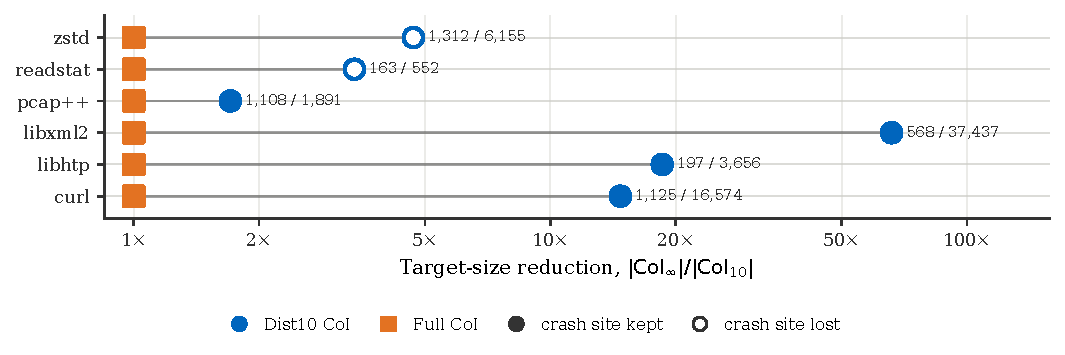
\includegraphics[width=\textwidth]{figures/rq1/coi-target-recall.pdf}
    \caption{Target size reduction and crash-site recall differences: Dist10-CoI vs. Full-CoI.}
    \label{fig:target_size_reduction}
\end{figure}

\paragraph{Target Area Size and Crash-Site Recall.}
The target size reduction and crash-site differences resulting from the distance-bounding ($\mathrm{CoI}_{10}$) policy are depicted in \cref{fig:target_size_reduction}.
Each project is presented separately with its reduction factor, the corresponding reduction in target lines of code, and whether the regression crash site is retained (filled circle) or excluded (hollow circle) by distance bounding.

Two main observations emerge.
First, the scale of target reduction depends heavily on the subject.
The observed reduction factors span from $\num{1.7}\times$ on \texttt{pcap++} up to $\num{66}\times$ on \texttt{libxml2}.
Across all subjects, bounding achieves a median target area reduction of $\num{9.7}\times$.
Thus, restricting the \ac{CoI} to a distance of \num{10} basic blocks from the change site yields orders-of-magnitude reductions in target static code size for most projects.
Second, this spatial reduction directly compromises defect safety.
For two targets, \texttt{zstd} and \texttt{readstat}, bounding the scope excludes the actual crash-site lines of the introduced regressions from the target set.
For these subjects, any coverage the pipeline achieves on the crash site is an indirect side effect of traversing the bounded region rather than a targeted objective.

\begin{figure}
    \centering
    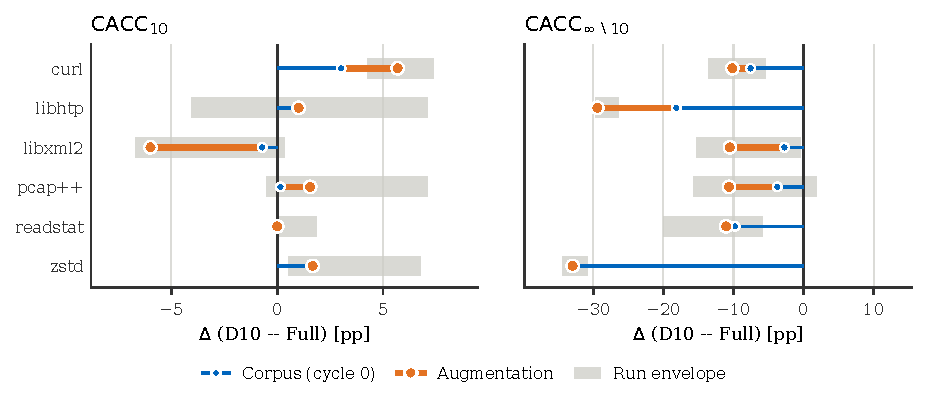
\includegraphics[width=\textwidth]{figures/rq1/cone-region-deltas.pdf}
    \caption{Median difference in \ac{CACC}: Dist10-CoI vs. Full-CoI}
    \label{fig:median_diff_coi_bound}
\end{figure}

\paragraph{Bounded and Complement Coverage.}
A reduced target scope is intended to focus the pipeline's synthesis effort, increasing coverage within the retained bounded region more effectively than an unbounded scope would.
The bounded ($\mathrm{CoI}_{10}$) and unbounded (Full) configurations, however, diverge at two stages: distillation already selects a different initial corpus (cycle~0), and the agent then pursues a different coverage target during augmentation.
\Cref{fig:median_diff_coi_bound} therefore splits the median difference for the near-change region ($\mathrm{CACC}_{10}$) and the complementary distant region ($\mathrm{CACC}_{\infty \setminus 10}$) into the part already present in the distilled corpus and the part added by augmentation.
\Cref{tab:coi_scope_score} details the statistical test results for the final corpora.

The bounded configuration yields a corpus that is markedly more concentrated in the near-change region.
Its distant coverage is lower across all projects, and the pooled difference is significant.
In \num{5} of the \num{6} projects, the separation is complete, with every bounded run ending below every unbounded run.
Only \texttt{pcap++} narrowly misses the significance threshold, because a single unbounded run ends level with the bounded median.
Much of this drop, however, stems from distillation rather than from the agent.
For \texttt{curl}, \texttt{libhtp}, \texttt{readstat}, and \texttt{zstd}, most of the gap is already present at cycle~0, and for \texttt{zstd} augmentation leaves it essentially unchanged.
Augmentation is the dominant contributor only for \texttt{libxml2} and \texttt{pcap++}.
For \texttt{curl}, \texttt{libhtp}, \texttt{libxml2}, and \texttt{zstd}, the bounded agent adds little distant coverage beyond its distilled corpus, whereas the unbounded agent continues to extend it.
For \texttt{pcap++} and \texttt{readstat}, in contrast, the bounded agent gains substantial distant coverage, nearly as much as the unbounded agent.
This suggests that inputs reaching the near-change code in these projects indirectly exercise large parts of the distant code.
Overall, the agent largely respects the boundary of its assigned target, but the magnitude of the drop is primarily due to the reduced initial corpus rather than to the agent's synthesis behavior.

Restricting the target scope, in contrast, yields negligible benefit within the bounded region itself.
The pooled gain in near-change coverage is small and not significant.
Separating the two stages shows that even this small gain is rarely attributable to more focused synthesis.
For \texttt{libhtp} and \texttt{zstd}, the entire difference is attributed to the distillation step, and both agents subsequently raise near-change coverage by the same amount.
The significant gain for \texttt{zstd}, therefore, originates from distillation, not from augmentation.
\texttt{readstat} shows no difference at either stage.
\texttt{pcap++} starts from nearly equivalent corpora, and both agents raise near-change coverage by similarly large amounts, leaving a small, non-significant difference.
Only \texttt{curl} exhibits a significant gain to which augmentation contributes meaningfully.
Roughly half of this gain is inherited from distillation, and the bounded agent adds the rest by extending its distilled corpus further than the unbounded agent does.
\texttt{libxml2} reverses the expected pattern.
Its distilled corpora are nearly equivalent, yet the bounded agent adds almost no near-change coverage, while the unbounded agent raises it substantially in several runs.
A possible explanation is that this near-change code is reachable via input structures that the bounded target does not incentivize.
For \texttt{libhtp}, \texttt{libxml2}, and \texttt{pcap++}, the per-run differences additionally span zero, indicating that run-to-run variation is of the same order as the observed effect.

\begin{table}
  \centering
  \def\rk#1{\,\textsuperscript{(#1)}}%
  \def\hd#1{\multicolumn{5}{c}{#1}}%
  \begin{threeparttable}
    \footnotesize
    \setlength{\tabcolsep}{3pt}
    \begin{tabular*}{\textwidth}{@{\extracolsep{\fill}}l cc c S[table-format=1.3] l cc c S[table-format=1.3] l@{}}
       & \hd{(1) $\mathrm{CACC}_{10}$ ($\uparrow$)} & \hd{(2) $\mathrm{CACC}_{\infty \setminus 10}$ ($\uparrow$)} \\
      \cmidrule(lr){2-6}\cmidrule(lr){7-11}
      \textbf{Project} & \textbf{CoI10} & \textbf{Full} & \textbf{$\Delta$} & {\textbf{$p_{Holm}$}} & {\textbf{$\hat A_{12}$}} & \textbf{CoI10} & \textbf{Full} & \textbf{$\Delta$} & {\textbf{$p_{Holm}$}} & {\textbf{$\hat A_{12}$}} \\
      \midrule
      curl & \textbf{74.7}\rk{1} & 69.0\rk{2} & $+$5.7 & {\textbf{0.048}} & 1.00 & 36.4\rk{2} & \textbf{46.6}\rk{1} & $-$10.2 & {\textbf{0.048}} & 0.00 \\
      libhtp & \textbf{93.9}\rk{1} & 92.9\rk{2} & $+$1.0 & 0.190 & 0.82 & 44.2\rk{2} & \textbf{73.6}\rk{1} & $-$29.4 & {\textbf{0.048}} & 0.00 \\
      libxml2 & 43.3\rk{2} & \textbf{49.3}\rk{1} & $-$6.0 & 0.063 & 0.04 & 7.3\rk{2} & \textbf{17.8}\rk{1} & $-$10.5 & {\textbf{0.048}} & 0.00 \\
      pcap++ & \textbf{85.6}\rk{1} & 84.1\rk{2} & $+$1.6 & 0.167 & 0.88 & 62.2\rk{2} & \textbf{72.8}\rk{1} & $-$10.6 & 0.056 & 0.12 \\
      readstat & \textbf{84.0}\rk{1} & \textbf{84.0}\rk{1} & $+$0.0 & 1.000 & 0.60 & 61.7\rk{2} & \textbf{72.8}\rk{1} & $-$11.1 & {\textbf{0.048}} & 0.00 \\
      zstd & \textbf{80.1}\rk{1} & 78.4\rk{2} & $+$1.7 & {\textbf{0.048}} & 1.00 & 31.0\rk{2} & \textbf{63.9}\rk{1} & $-$33.0 & {\textbf{0.048}} & 0.00 \\
      \midrule
      \textbf{All projects} & \textbf{82.1}\rk{1.17} & 81.2\rk{1.67} & $+$1.0 & 0.625 & 4W 1T 1L & 40.3\rk{2.00} & \textbf{68.3}\rk{1.00} & $-$19.8 & {\textbf{0.031}} & 0W 0T 6L \\
      \bottomrule
    \end{tabular*}
    \caption{Scoring of \ac{CoI} scoping effectiveness}
    \label{tab:coi_scope_score}
  \end{threeparttable}
\end{table}

\paragraph{\ac{CoI} Scope Decision.}
Overall, while the bounded configuration concentrates coverage within the local neighborhood of the change site, it fails to meaningfully improve coverage in that local region compared with an unbounded scope.
Simultaneously, it penalizes safety by excluding known regression crash sites and severely reducing coverage across the surrounding context.
Following the decision rule, the \emph{full} \ac{CoI} scope is selected for the pipeline to preserve safety and complement coverage without sacrificing local reachability.

\subsection{Discussion}
The findings from both seed augmentation studies highlight key trade-offs in configuring the augmentation pipeline.

\paragraph{Starting Corpus Composition.}
Supplying more seeds to the agent does not monotonically improve LLM-guided seed generation.
Even when starting from an empty reference corpus, the agent closely matches the change-affected code coverage of the resulting corpora, relying solely on inference over code semantics.
However, when a project already maintains a well-engineered corpus, as is the case for \texttt{curl} and \texttt{zstd}, the agent cannot match the value embedded in these hand-crafted inputs without access to them.
This underlines the value of building upon existing corpus knowledge whenever it is available.
Distillation offers an effective middle ground: it reduces the often massive original base corpora to a manageable set while still yielding improvements over that initial set.
The cost of this reduction is that coverage-based distillation cannot judge structural diversity and therefore discards information the agent could otherwise build upon.
This effect is visible for \texttt{curl}, where the final coverage achieved when starting from the original corpus exceeded that of the distilled starting corpus.
Inputs that do not reach the change region may nonetheless be structurally close to relevant ones, and thus serve as valuable templates from which the agent can derive change-targeted seeds.

\paragraph{Static Target Granularity vs.\ Semantic Relevance.}
% TODO: Finalize once the decomposition of distillation vs. LLM contribution is available.
Constraining the static target scope sharpens the focus of LLM-guided synthesis, but spatial concentration does not translate directly into higher coverage within the targeted region.
Distillation is an effective tool for making seeds more targeted, as it selects only those seeds that reach the target area.
More critically, restricting the static scope based purely on basic-block distance risks truncating control-flow paths that contain the true root causes or crash locations of regressions.
The distance threshold in the CoI-Fuzzer tool could be increased, but doing so defeats the purpose of bounding the scope in the first place.
While further truncation policies are implemented, none of them achieves a substantial reduction in scope while maintaining adequate safety.
Further research to define a safe subset of the full \ac{CoI} would therefore be valuable and further improve the presented pipeline.

\paragraph{Practical Pipeline Configuration.}
Together, these results reveal an asymmetric design principle for change-targeted seed generation: pipelines should be selective about the seeds supplied to the LLM, but conservative about the code scope considered relevant to the change.
Restricting the seed corpus via distillation reduces noise and context bloat during synthesis, while maintaining the full \ac{CoI} scope ensures that potential defect sites remain visible.
Consequently, carrying the \emph{distilled} starting corpus alongside the \emph{full} \ac{CoI} scope into end-to-end fuzzing campaigns provides the most effective baseline for downstream vulnerability discovery.

\section{Fuzzing Study}\label{sec:eval:fuzzing}
The second study evaluates the resulting corpus in an end-to-end fuzzing campaign, comparing the LLM-augmented corpus produced by the configuration selected in \rqref{1.1} and \rqref{1.2} against the project's original corpus.
It addresses the following research questions:

\begin{description}
  \item[\researchq{2.1} (reliability)] How often do campaigns seeded with each corpus expose the target regression bug within the campaign budget, with and without accounting for seed augmentation overhead??
  \item[\researchq{2.2} (generalization)] Does the detection rate on the subjects used to select the configuration differ from that on the held-out subjects?
  \item[\researchq{2.3} (efficiency)] How does the expected time-to-exposure of the target bug within the campaign budget differ between the two seed corpora, with and without accounting for seed augmentation overhead?
  \item[\researchq{2.4} (attribution)] What factors in the seed augmentation pipeline account for differences in regression exposure between campaigns using the augmented corpus and the baseline corpus?
\end{description}

Together, the research questions establish whether the gains observed in the seed generation study translate to an end-to-end fuzzing campaign and whether they hold for subjects who played no part in selecting the configuration.

\subsection{Subjects}\label{sec:eval:fuzzing:subjects}
This study uses all \num{12} subjects introduced in \autoref{sec:eval:subjects}.
\num{6} subjects were used to select the configuration in \autoref{sec:eval:seedgen}; the remaining \num{6} played no part in that selection and serve to expose any overfitting of the configuration to the selection set.
This split is marked in every per-subject table and plot, so that it remains visible whether an observed effect is confined to the subjects that informed the configuration.

Aggregate figures and statistical tests are computed over the full set of \num{12}; the split is not treated as a factor.
On \num{4} of the \num{6} held-out subjects, neither corpus exposed the bug within the budget, leaving too few informative subjects for a separate comparison.

\subsection{Procedure}\label{sec:eval:fuzzing:procedure}
Each subject is fuzzed under two arms: seeded with the project's original corpus, and seeded with the LLM-augmented corpus produced by the configuration selected in \autoref{sec:eval:seedgen}.
Corpus augmentation is performed once per subject, so the only source of randomness within an arm is the fuzzing campaign itself.
For the tuning set, the latest result from the \num{5} runs is evaluated in \cref{sec:eval:seedgen} to save costs, whereas for the held-out set, a single augmentation run was performed independently.
Costs are reported in \cref{tab:termination-fuzzing} but not evaluated within the scope of this study.

The campaign budget is \SI{8}{\hour}, the longest campaign that still fits an overnight CI/CD run~\cite{kloosterEffectivenessScalabilityFuzzing2022}.
This is shorter than the \SI{24}{\hour} convention common in fuzzer evaluations~\cite{klees2018}, and the trade-off runs in a direction that favors the technique under test: a short budget rewards seeds that pay off early, which is precisely what per-commit regression-targeted corpus augmentation is designed to produce.
This is stated explicitly rather than treating \SI{8}{\hour} as neutral, and revisited in \autoref{sec:eval:threats}.

Every arm is run for \num{10} independent campaigns per subject, each with a distinct fuzzer seed and no state shared between runs.
A campaign counts as a reproduction only when the crash matches the target regression: BugOSS supplies the bug-revealing input along with the bug, and a match is confirmed manually against the sanitizer report and the faulting location, rather than counting arbitrary crashes by matching the top frames of the call stack and their line numbers.

\paragraph{Unit of analysis.}
Campaigns are not pooled across subjects.
Corpus construction is performed once per subject, so the \num{10} campaigns within a subject are repeated measurements of one constructed corpus rather than independent samples of the technique, and the subject is the unit of analysis for every cross-subject statement.
Within a subject, the \num{10} campaigns are independent and are compared directly.

\paragraph{Time to Error.}
Campaigns that reach the budget without reproducing the bug have no \ac{TTE}.
These are treated as right-censored at \SI{8}{\hour} rather than discarded or imputed, following Magma~\cite{hazimehMagmaGroundTruthFuzzing2020}.
Each subject and arm is summarized by the \ac{RMST} at the \SI{8}{\hour} horizon: the average time for which the bug survives undetected over a campaign capped at \SI{8}{\hour}, computed as the area under the Kaplan--Meier estimate.
\ac{RMST} is defined for every subject, including those where fewer than half the campaigns reproduce the bug, and the median \ac{TTE} does not exist.
All reported \ac{RMST} values are relative to the \SI{8}{\hour} budget and are not comparable to figures obtained under a different horizon.
Statistical comparisons follow the continuous-outcome procedure for two arms in \autoref{sec:eval:statistics}.

\paragraph{Reproduction Rate.}
\ac{RMST} is the primary outcome of this study; the reproduction rate is the endpoint of the same survival curve and is reported as a reliability view of it, rather than as stand-alone evidence.
Reproduction rates are reported per subject as the fraction of campaigns exposing the bug, together with the mean rate per arm; statistical comparisons follow the binary-outcome procedure for two arms in \autoref{sec:eval:statistics}.

\paragraph{Case Attribution.}
\rqref{2.4} is answered by a post-hoc case attribution analysis in two steps: case selection, then tracing where the regression-exposing inputs came from.

First, the subjects that show suggestive evidence of a difference in \ac{RMST} between the arms, in either direction, are selected.
With only \num{10} campaigns per arm, the conventional threshold of $p < \num{0.05}$ would discard differences that are large but uncertain.
For selection, the threshold is therefore raised to $p_{Holm} < \num{0.15}$.
This is a filter for which subjects to explain, not a significance claim.
It excludes the \num{4} subjects without any exposure and the \num{3} subjects whose difference is indistinguishable from noise (\emph{libhtp}, \emph{readstat}, \emph{openssl}).
\num{5} subjects remain: \emph{yara}, \emph{pcap++}, \emph{libxml2}, \emph{zstd}, and \emph{curl}, of which only \emph{pcap++} is not significant at \num{0.05}.

Second, the provenance of the regression-exposing inputs is traced.
For every campaign, the \emph{first} crash that matches the target regression is taken.
As with \ac{RMST}, crashes after the \SI{8}{\hour} horizon do not count.
AFL++ records, for each queue entry, the entry it was mutated from.
These links are followed back to the corpus file the crash descends from, termed its \emph{ancestor}, and the number of queue entries on the way is termed its number of \emph{generations}.
Each unique ancestor is then located in the corpus stages of the pipeline (\cref{tab:attribution}):
\begin{description}
  \item[Baseline ancestors] unique ancestors of the original arm, over the
    size of the original corpus;
  \item[Distilled] unique ancestors of the augmented arm that were already
    in the distilled corpus, over its size;
  \item[Generated] unique ancestors of the augmented arm that entered the
    corpus after distillation, over the number of files added after it.
  \item[Final corpus] the union of both, over the size of the corpus, the augmented fuzzing campaigns were seeded with.
\end{description}
\emph{Crash} marks an arm whose corpus already reproduced the regression during pre-fuzzing screening, so the campaigns never had to fuzz.
Each case is then read through its ancestors, the files themselves, where needed, and the generation counts.
Finally, the cases are grouped by which stage supplied the exposing input.
The attribution shows which seed a crash actually descends from.
It does not show that any other seed could have led to the crash.
It explains the observed difference, but it is not a counterfactual.

\subsection{Results}
\begin{figure}
  \centering
  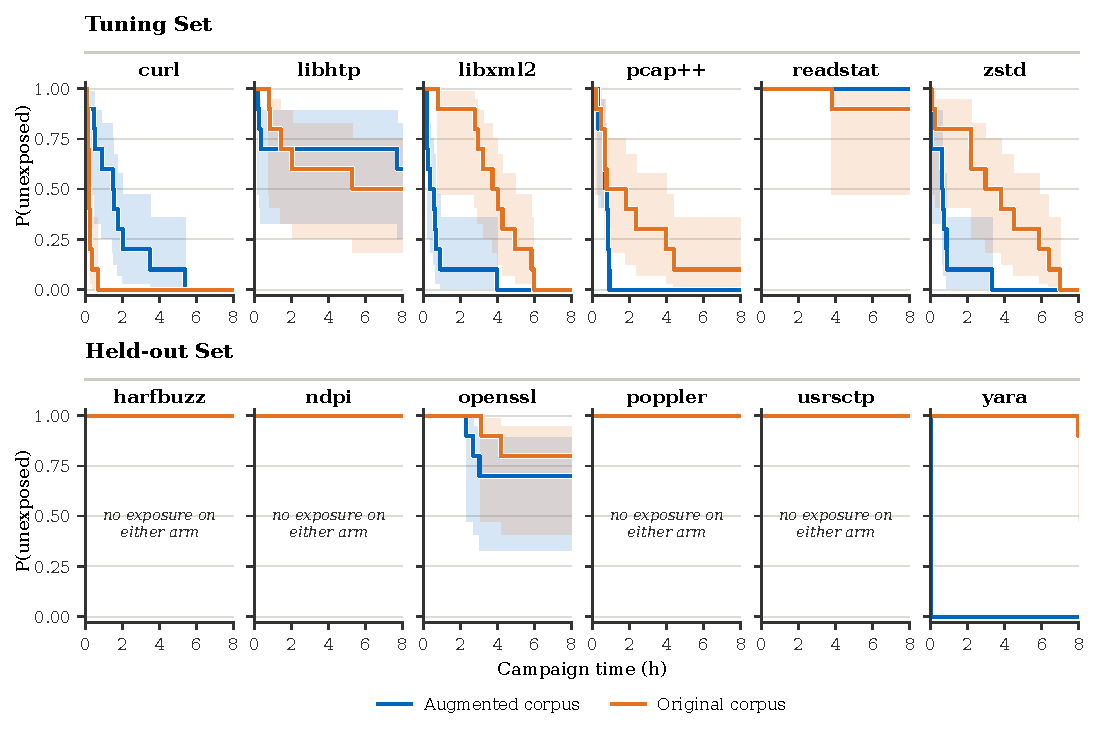
\includegraphics[width=\textwidth]{figures/bug-survival-curves.pdf}
  \caption[Bug Survival Curves]{%
    Kaplan--Meier estimate bug survival curves, one tile per project, with error bands.
  \label{fig:bug_survival_curves}
  }
\end{figure}

\Cref{fig:bug_survival_curves} summarizes the campaign outcomes as subject-level survival curves over the \SI{8}{\hour} horizon, one panel per subject with a separate curve per arm.
Higher curves mean the bug survived longer, and steep drops mark reproductions.
The \num{4} held-out subjects that yielded no exposure at all remain flat at \num{1.0} across the horizon, while \emph{yara}'s augmented arm starts at \num{0.0} because its corpus already contained a bug-exposing input before fuzzing began.
Numeric summaries derived from these curves are reported alongside each research question below.

\begin{table}
  \centering
  \def\rk#1{\,\textsuperscript{(#1)}}%
  \def\hd#1{\multicolumn{4}{c}{#1}}%
  \begin{threeparttable}
    \footnotesize
    \setlength{\tabcolsep}{3pt}
    \begin{tabular*}{\textwidth}{@{\extracolsep{\fill}}l cc c S[table-format=1.3] cc c S[table-format=1.3]@{}}
      \textbf{Reproduction rate ($\uparrow$)} & \hd{(1) Without overhead} & \hd{(2) With overhead} \\
      \cmidrule(lr){2-5}\cmidrule(lr){6-9}
      \textbf{Project} & \textbf{Augmented} & \textbf{Original} & \textbf{$\Delta$} & {\textbf{$p_{Holm}$}} & \textbf{Augmented} & \textbf{Original} & \textbf{$\Delta$} & {\textbf{$p_{Holm}$}} \\
      \midrule
      \addlinespace[2pt]
      \multicolumn{9}{@{}l}{\textsc{Tuning set}\ \textnormal{(6 projects)}} \\
      \addlinespace[1pt]
      \hspace{1em}curl & 1.00\rk{1} & 1.00\rk{1} & \phantom{$+$}0.00 & {--} & 1.00\rk{1} & 1.00\rk{1} & \phantom{$+$}0.00 & {--} \\
      \hspace{1em}libhtp & 0.40\rk{2} & \textbf{0.50}\rk{1} & $-$0.10 & 1.000 & 0.30\rk{2} & \textbf{0.50}\rk{1} & $-$0.20 & 1.000 \\
      \hspace{1em}libxml2 & 1.00\rk{1} & 1.00\rk{1} & \phantom{$+$}0.00 & {--} & 1.00\rk{1} & 1.00\rk{1} & \phantom{$+$}0.00 & {--} \\
      \hspace{1em}pcapplusplus & \textbf{1.00}\rk{1} & 0.90\rk{2} & $+$0.10 & 1.000 & \textbf{1.00}\rk{1} & 0.90\rk{2} & $+$0.10 & 1.000 \\
      \hspace{1em}readstat & 0.00\rk{2} & \textbf{0.10}\rk{1} & $-$0.10 & 1.000 & 0.00\rk{2} & \textbf{0.10}\rk{1} & $-$0.10 & 1.000 \\
      \hspace{1em}zstd & 1.00\rk{1} & 1.00\rk{1} & \phantom{$+$}0.00 & {--} & 1.00\rk{1} & 1.00\rk{1} & \phantom{$+$}0.00 & {--} \\
      \addlinespace[6pt]
      \multicolumn{9}{@{}l}{\textsc{Held-out set}\ \textnormal{(6 projects)}} \\
      \addlinespace[1pt]
      \hspace{1em}harfbuzz & 0.00\rk{1} & 0.00\rk{1} & \phantom{$+$}0.00 & {--} & 0.00\rk{1} & 0.00\rk{1} & \phantom{$+$}0.00 & {--} \\
      \hspace{1em}ndpi & 0.00\rk{1} & 0.00\rk{1} & \phantom{$+$}0.00 & {--} & 0.00\rk{1} & 0.00\rk{1} & \phantom{$+$}0.00 & {--} \\
      \hspace{1em}openssl & \textbf{0.30}\rk{1} & 0.20\rk{2} & $+$0.10 & 1.000 & \textbf{0.30}\rk{1} & 0.20\rk{2} & $+$0.10 & 1.000 \\
      \hspace{1em}poppler & 0.00\rk{1} & 0.00\rk{1} & \phantom{$+$}0.00 & {--} & 0.00\rk{1} & 0.00\rk{1} & \phantom{$+$}0.00 & {--} \\
      \hspace{1em}usrsctp & 0.00\rk{1} & 0.00\rk{1} & \phantom{$+$}0.00 & {--} & 0.00\rk{1} & 0.00\rk{1} & \phantom{$+$}0.00 & {--} \\
      \hspace{1em}yara & \textbf{1.00}\rk{1} & 0.10\rk{2} & $+$0.90 & {\textbf{$<$0.001}} & \textbf{1.00}\rk{1} & 0.10\rk{2} & $+$0.90 & {\textbf{$<$0.001}} \\
      \midrule
      \textbf{All projects} & \textbf{0.48}\rk{1.17} & 0.40\rk{1.25} & \phantom{$+$}0.00 & 1.000 & \textbf{0.47}\rk{1.17} & 0.40\rk{1.25} & \phantom{$+$}0.00 & 1.000 \\
      \bottomrule
    \end{tabular*}
    \caption{Fuzzing crash reproduction rate across subjects.}\label{tab:bugeval-reproduction}
  \end{threeparttable}
\end{table}


\begin{tcolorbox}[colback=black!4, colframe=black!40, boxrule=0.4pt,
                  left=6pt, right=6pt, top=6pt, bottom=6pt]
\rqref{2.1} Across the \num{12} subjects, the augmented corpus reproduced the regression more often in three, less often in two and equally often in seven (\SI{48}{\percent} vs.\ \SI{40}{\percent} of campaigns, \SI{47}{\percent} with the pipeline overhead charged), a median paired difference of zero that is not significant with or without the overhead ($p = \num{1.00}$).
\end{tcolorbox}


Per-subject reproduction rates are reported in \cref{tab:bugeval-reproduction}.
Only \emph{yara} separates the arms within a subject after Holm adjustment:
its augmented corpus exposed the bug in all \num{10} campaigns, against \num{1} of \num{10} for the original corpus.
The remaining differences are one-campaign-wide, and none are significant.

The seven tied subjects are tied for two opposite reasons, and the distinction matters for the rest of this section.
Four of them (\emph{harfbuzz}, \emph{ndpi}, \emph{poppler}, \emph{usrsctp}) produced no exposure in either arm, so the measure has nothing to separate.
The other three (\emph{curl}, \emph{libxml2}, \emph{zstd}) reproduced the bug in \emph{every} campaign of \emph{both} arms, so the reproduction rate is saturated at \num{1.00} and cannot express a difference that exists.
As \cref{tab:bugeval-rmst} shows, all three of these subjects separate clearly on time to exposure.
The reproduction rate is therefore reported here as a reliability view of the survival curve rather than as the efficiency measure, and \ac{RMST} is the primary outcome.

When accounting for the overhead introduced by the pipeline, only one exposure on \emph{libhtp} exceeded the adjusted \SI{8}{\hour} window, reducing its augmented reproduction rate from \num{0.40} to \num{0.30}.
All other rates are unchanged: every other augmented exposure still fell inside the window after its subject's overhead was added, which ranges from about \SI{45}{\minute} to \SI{2.75}{\hour} (\cref{tab:bugeval-rmst}).
The overhead, therefore, leaves the reproduction picture intact.
\emph{yara} remains the only subject that separates the arms, and the pooled sign test stays at $p = \num{1.000}$.

\begin{tcolorbox}[colback=black!4, colframe=black!40, boxrule=0.4pt,
                  left=6pt, right=6pt, top=6pt, bottom=6pt]
\rqref{2.2} Generalization to the held-out subjects remains inconclusive: on \num{4} of the \num{6} neither corpus exposed the bug within the budget, leaving \num{2} informative subjects, one of which reflects a corpus that already contained a bug-exposing input before fuzzing began.
\end{tcolorbox}

Of the \num{6} held-out subjects, \emph{harfbuzz}, \emph{ndpi}, \emph{poppler} and \emph{usrsctp} produced no reproduction in either arm across all \num{20} campaigns, so neither the reproduction rate nor the \ac{TTE} can distinguish the corpora there.
The two remaining subjects are \emph{yara} and \emph{openssl}.
\emph{Yara}'s effect is the largest in the study but does not measure fuzzing at all: the augmented corpus contained an input that crashed the target before the first campaign second, so the comparison records corpus construction rather than search.
Setting it aside leaves \emph{openssl}, whose advantage is \num{1} campaign in \num{10} and not significant.
No claim about generalization is supported in either direction by this evidence.

\begin{table}
  \centering
  \def\rk#1{\,\textsuperscript{(#1)}}%
  \def\hd#1{\multicolumn{4}{c}{#1}}%
  \begin{threeparttable}
    \footnotesize
    \setlength{\tabcolsep}{3pt}
    \begin{tabular*}{\textwidth}{@{\extracolsep{\fill}}l cc c S[table-format=1.3] cc c S[table-format=1.3]@{}}
      \textbf{$RMST_{8h}$ (h:mm) ($\downarrow$)} & \hd{(1) Without overhead} & \hd{(2) With overhead} \\
      \cmidrule(lr){2-5}\cmidrule(lr){6-9}
      \textbf{Project} & \textbf{Augmented} & \textbf{Original} & \textbf{$\Delta$} & {\textbf{$p_{Holm}$}} & \textbf{Augmented} & \textbf{Original} & \textbf{$\Delta$} & {\textbf{$p_{Holm}$}} \\
      \midrule
      \addlinespace[2pt]
      \multicolumn{9}{@{}l}{\textsc{Tuning set}\ \textnormal{(6 projects)}} \\
      \addlinespace[1pt]
      \hspace{1em}curl & 1:45\rk{2} & \textbf{0:14}\rk{1} & $+$1:30 & {\textbf{0.005}} & 2:51\rk{2} & \textbf{0:14}\rk{1} & $+$2:37 & {\textbf{$<$0.001}} \\
      \hspace{1em}libhtp & 5:38\rk{2} & \textbf{5:02}\rk{1} & $+$0:36 & 1.000 & 5:54\rk{2} & \textbf{5:02}\rk{1} & $+$0:51 & 1.000 \\
      \hspace{1em}libxml2 & \textbf{0:47}\rk{1} & 3:50\rk{2} & $-$3:02 & {\textbf{0.003}} & \textbf{2:08}\rk{1} & 3:50\rk{2} & $-$1:41 & 0.082 \\
      \hspace{1em}pcapplusplus & \textbf{0:41}\rk{1} & 2:19\rk{2} & $-$1:37 & 0.130 & \textbf{1:30}\rk{1} & 2:19\rk{2} & $-$0:48 & 1.000 \\
      \hspace{1em}readstat & 8:00\rk{2} & \textbf{7:34}\rk{1} & $+$0:25 & 1.000 & 8:00\rk{2} & \textbf{7:34}\rk{1} & $+$0:25 & 1.000 \\
      \hspace{1em}zstd & \textbf{0:46}\rk{1} & 3:30\rk{2} & $-$2:44 & {\textbf{0.020}} & \textbf{1:49}\rk{1} & 3:30\rk{2} & $-$1:41 & 0.281 \\
      \addlinespace[6pt]
      \multicolumn{9}{@{}l}{\textsc{Held-out set}\ \textnormal{(6 projects)}} \\
      \addlinespace[1pt]
      \hspace{1em}harfbuzz & 8:00\rk{1} & 8:00\rk{1} & \phantom{$+$}0:00 & {--} & 8:00\rk{1} & 8:00\rk{1} & \phantom{$+$}0:00 & {--} \\
      \hspace{1em}ndpi & 8:00\rk{1} & 8:00\rk{1} & \phantom{$+$}0:00 & {--} & 8:00\rk{1} & 8:00\rk{1} & \phantom{$+$}0:00 & {--} \\
      \hspace{1em}openssl & \textbf{6:23}\rk{1} & 7:07\rk{2} & $-$0:43 & 1.000 & 7:13\rk{2} & \textbf{7:07}\rk{1} & $+$0:05 & 1.000 \\
      \hspace{1em}poppler & 8:00\rk{1} & 8:00\rk{1} & \phantom{$+$}0:00 & {--} & 8:00\rk{1} & 8:00\rk{1} & \phantom{$+$}0:00 & {--} \\
      \hspace{1em}usrsctp & 8:00\rk{1} & 8:00\rk{1} & \phantom{$+$}0:00 & {--} & 8:00\rk{1} & 8:00\rk{1} & \phantom{$+$}0:00 & {--} \\
      \hspace{1em}yara & \textbf{0:00}\rk{1} & 7:59\rk{2} & $-$7:59 & {\textbf{$<$0.001}} & \textbf{0:56}\rk{1} & 7:59\rk{2} & $-$7:03 & {\textbf{$<$0.001}} \\
      \midrule
      \textbf{All projects} & \textbf{4:40}\rk{1.25} & 5:48\rk{1.42} & $-$1:11 & 0.148 & \textbf{5:11}\rk{1.33} & 5:48\rk{1.33} & $-$0:31 & 0.641 \\
      \bottomrule
    \end{tabular*}
    \caption{Fuzzing \ac{RMST} across subjects.}\label{tab:bugeval-rmst}
  \end{threeparttable}
\end{table}

\begin{tcolorbox}[colback=black!4, colframe=black!40, boxrule=0.4pt,
                  left=6pt, right=6pt, top=6pt, bottom=6pt]
\rqref{2.3} Across the \num{12} subjects, the augmented corpus reduced \ac{RMST} in \num{5}, increased it in \num{3}, and left it unchanged in \num{4}, with a median paired difference of \SI{71}{\minute} during fuzzing execution and \SI{31}{\minute} once the augmentation overhead is charged to each campaign (neither significant, $p = \num{0.148}$ and $p = \num{0.641}$).
\end{tcolorbox}

\Cref{tab:bugeval-rmst} reports \ac{RMST} per subject and arm.
\num{4} subjects separate after Holm adjustment.
Three favor augmentation (\texttt{yara}, \texttt{libxml2}, and \texttt{zstd}) and one favors the original corpus: \texttt{curl} exposed the bug \SI{1}{\hour}\,\SI{31}{\minute} later under augmentation.
Of the remaining subjects, \texttt{pcap++} and \texttt{openssl} favor augmentation, and \emph{libhtp} and \emph{readstat} the original, none significantly, and \num{4} admit no test because neither arm ever exposed the bug.

\begin{figure}
  \centering
  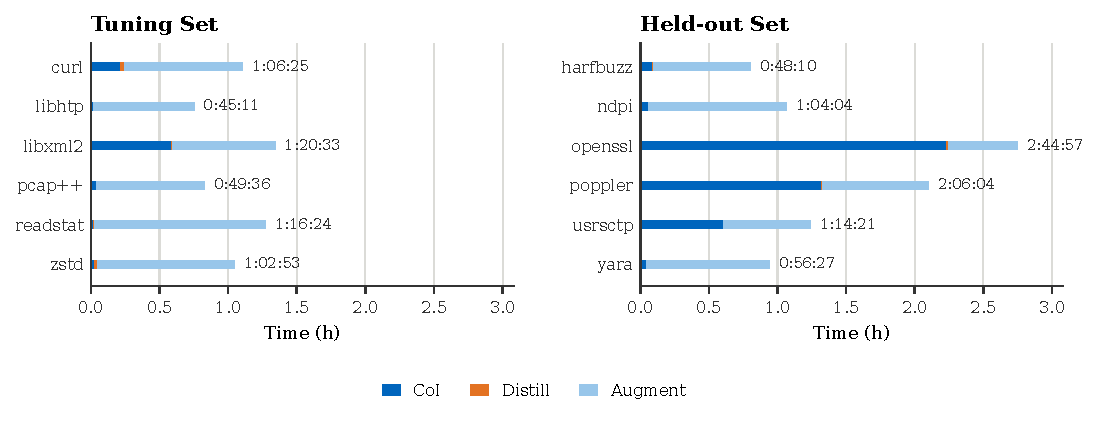
\includegraphics[width=\textwidth]{figures/augmentation-overhead.pdf}
  \caption{Time overhead of TACCO's augmentation stage}
  \label{fig:aug_overhead}
\end{figure}

Charging every augmented campaign with the wall-clock cost of the augmentation pipeline (\cref{fig:aug_overhead}) before applying the horizon shifts the split from five--four--three to four--four--four and shrinks the median paired difference from \SI{71}{\minute} to \SI{31}{\minute}, at which point the difference is no longer significant ($p = \num{0.641}$).
The overhead comes mainly from two phases.
The \ac{LLM} agent augmentation phase has a fairly consistent duration across projects, with a median of \SI{41}{\minute}.
The duration of the \ac{CoI} computation phase depends on project size, with a median of \SI{4.5}{\minute} and a range from \SI{1}{\minute} (\texttt{libhtp}) to \SI{134}{\minute} (\texttt{openssl}).
The overhead introduced by distillation is negligible in this context, with a maximum runtime of \SI{204}{\second} for \texttt{curl}.

\begin{tcolorbox}[colback=black!4, colframe=black!40, boxrule=0.4pt,
                  left=6pt, right=6pt, top=6pt, bottom=6pt]
\rqref{2.4} Exposure differences trace back to the pipeline's two stages, whose effects can reinforce or offset each other.
\begin{itemize}
  \item \textbf{Distillation} speeds up exposure by concentrating the budget on an ancestor that the original corpus already had (\emph{zstd}, \emph{libxml2}).
    It slows exposure by discarding the original corpus's close representatives of the required structure (\emph{curl}).
  \item \textbf{Generation} speeds up exposure when it supplies a structure the original corpus lacked entirely (\emph{yara}, \emph{pcap++}).
    It only partly compensates when it reconstructs what distillation dropped (\emph{curl}).
\end{itemize}
\end{tcolorbox}

\begin{table}
  \centering
  \begin{threeparttable}
    \footnotesize
    \setlength{\tabcolsep}{6pt}
    \sisetup{group-separator = {,}, group-minimum-digits = 4}
    \begin{tabular}{l l
                    S[table-format=5.0]
                    S[table-format=2.0]
                    S[table-format=3.0]
                    S[table-format=3.0]
                    r}
      \toprule
      \textbf{Project} & &  & \multicolumn{3}{c}{\textbf{Pipeline}} & \\
      \cmidrule(lr){4-6}
       & & {\textbf{Baseline}} & {\textbf{Distilled}} & {\textbf{Generated}} & {\textbf{Final corpus}} & \textbf{$\Delta$ RMST} \\
      \midrule
      \multirow{2}{*}{yara}    & \textit{unique ancestors} & 1     & 0  & 3   & \multicolumn{1}{c}{\multirow{2}{*}{\textit{Crash}}} & \multirow{2}{*}{$-$7:59:50} \\
                               & \textit{corpus size}      & 9     & 5  & 100 &     & \\
      \addlinespace
      \multirow{2}{*}{pcap++}  & \textit{unique ancestors} & 5     & 0  & 5   & 5   & \multirow{2}{*}{$-$1:37:50} \\
                               & \textit{corpus size}      & 615   & 25 & 505 & 530 & \\
      \addlinespace
      \multirow{2}{*}{libxml2} & \textit{unique ancestors} & 9     & 1  & 0   & 1   & \multirow{2}{*}{$-$3:02:25} \\
                               & \textit{corpus size}      & 1309  & 10 & 392 & 402 & \\
      \addlinespace
      \multirow{2}{*}{zstd}    & \textit{unique ancestors} & 5     & 1  & 0   & 1   & \multirow{2}{*}{$-$2:44:49} \\
                               & \textit{corpus size}      & 12462 & 25 & 91  & 116 & \\
      \addlinespace
      \multirow{2}{*}{curl}    & \textit{unique ancestors} & 8     & 1  & 7   & 8   & \multirow{2}{*}{$+$1:30:45} \\
                               & \textit{corpus size}      & 4202  & 30 & 478 & 508 & \\
      \bottomrule
    \end{tabular}
    \caption{Attribution results for the five selected subjects.}\label{tab:attribution}
  \end{threeparttable}
\end{table}

\Cref{tab:attribution} gives, for each selected subject, the corpus stage from which its exposing inputs descend.
The cases are discussed in the order of the attribution patterns they form.

\paragraph{pcap++.}
PcapPlusPlus is a C++ library for capturing and parsing network traffic; its fuzz target decodes each protocol layer of a packet capture (\texttt{.pcap} file).
The regression concerns the TLS \emph{CertificateRequest}, a handshake message in which a server asks for a client certificate.
Here, the pipeline's advantage comes from generation: the original corpus contains no TLS handshake at all, so no distillation could have preserved one.
All augmented campaigns descend from \num{5} agent-written captures, half of them from \texttt{ssl\_certreq\_clamp.pcap}.
This seed is a minimal, valid CertificateRequest with deliberately inconsistent content, announcing \num{255} certificate types in a message only \SI{2}{\byte} long.
From it, a single generation sufficed: every descending crash zeroes the low byte of the length field, and in one campaign that byte is the only difference between seed and crash.
The baseline campaigns reached the same crash from captures of unrelated protocols, but first spent \numrange{6}{18} generations building a valid TLS record.
As a result, the gain lies in reliability rather than typical speed.
Median time to exposure is almost equal, but all pipeline campaigns exposed the bug within \SI{55}{\minute}, whereas the slowest baseline campaign took \SI{4.4}{\hour}, and one never exposed it, which accounts for the difference in \ac{RMST}.
Distillation played no role: \num{4} of the \num{5} baseline ancestors survived it, yet no pipeline campaign descends from them, because the generated seeds were much closer to the crash.
This difference is attributed to generation.

\paragraph{yara.}
YARA is a pattern-matching tool used to classify malware; its PE module parses Windows executables (the Portable Executable format), and the regression lies in how it handles section names.
This is the most extreme case: the pipeline exposed the bug before fuzzing began.
During pre-fuzzing screening, \num{3} agent-written PE32 files, none of which were in the original corpus, had already reproduced it.
The original corpus, by contrast, led to the bug in only \num{1} of \num{10} campaigns, after \SI{7.97}{\hour} and \num{9} generations.
Distillation kept that test case, so the pipeline lost nothing, while generation added inputs that required no fuzzing at all; hence, $\Delta$~\ac{RMST} spans almost the entire horizon.
As noted for \rqref{2.2}, this case measures corpus construction rather than search.
This difference is attributed to generation.

\paragraph{libxml2.}
libxml2 is a widely used XML parser.
Here the pipeline did not bring the exposing input closer to the crash; it made that input far more likely to be fuzzed.
All augmented campaigns descend from one original seed, \texttt{ent\_738805.xml}, an XML document with entity declarations that distillation kept and that lies \numrange{2}{6} generations from the crash.
\num{9} of the pipeline campaigns exposed the bug within \SI{54}{\minute}.
In the baseline, the one campaign that descends from the same seed was just as fast (\SI{47}{\minute}, \num{3} generations).
The other \num{9} started from seeds that distillation dropped, needing up to \num{30} generations and a median of \SI{3.9}{\hour}.
The difference is in scheduling: after distillation, the exposed seed was \num{1} of \num{402} files rather than \num{1} of \num{1309}.
Generation contributed nothing, as none of the \num{392} \ac{LLM}-generated files are ancestors.
This difference is attributed to distillation.

\paragraph{zstd.}
zstd is a compression library implementing the Zstandard format; its fuzz target decompresses arbitrary input.
zstd shows the same mechanism as libxml2 more clearly: the bug is easy to reach from the original corpus, but the exposing seeds are buried in it.
The baseline had \num{5} ancestors, each only \numrange{1}{4} generations from the crash, yet needed a median of \SI{3.4}{\hour} (at most \SI{7.0}{\hour}), because AFL++ spreads its schedule over \num{12462} files.
Distillation dropped all \num{5} but kept a sixth original seed that is just as close.
All \num{10} pipeline campaigns descend from it within \numrange{1}{2} generations, with a median of \SI{39}{\minute}; \num{3} exposed the bug within the first minute.
Again, generation played no role: none of the \num{91} added files are ancestors, and the pipeline's ancestors are not closer to the crash (median \num{2} generations vs.\ \num{1}).
This difference is attributed to distillation.

\paragraph{curl.}
curl is a library and command-line tool for transferring data over protocols such as HTTP; its fuzz target replays scripted client--server exchanges.
curl is the only selected subject on which the pipeline was slower, because distillation removed the seeds closest to the bug and generation only partly replaced them.
The original corpus represents the exposing structure widely: all \num{10} baseline campaigns exposed the bug within \SI{41}{\minute} (median \SI{12}{\minute}), each \numrange{1}{2} generations from one of \num{8} distinct seeds.
Distillation dropped all \num{8}.
The one remaining original ancestor led a single pipeline campaign to the bug, after \num{4} generations and \SI{3.5}{\hour}.
The other \num{9} campaigns descend from \num{7} agent-written HTTP exchanges centered on redirects and authentication.
The agent thus aimed at the right functionality, but its seeds lie \numrange{1}{10} generations from the crash rather than \numrange{1}{2}, resulting in a median of \SI{1.5}{\hour} and a maximum of \SI{5.4}{\hour}.
This difference is attributed to distillation and is only partly offset by generation.

% ===================================================================
% (C) Results: synthesis
% ===================================================================

\paragraph{Synthesis.}
\Cref{tab:attribution-patterns} groups the five cases into three attribution patterns.

\begin{table}[t]
  \centering
  \begin{threeparttable}
    \footnotesize
    \begin{tabular}{p{0.24\linewidth} l p{0.20\linewidth} l l}
      \toprule
      \textbf{Pattern} & \textbf{Subjects} & \textbf{Augmented ancestors}
        & \textbf{Gens.\ to crash}\tnote{a} & \textbf{Exposure}\tnote{a} \\
      \midrule
      Distillation concentrates budget on an existing seed
        & \emph{zstd}, \emph{libxml2}
        & Distilled originals only
        & No closer
        & Faster \\
      \addlinespace
      Generation adds structure missing from the corpus
        & \emph{yara}, \emph{pcap++}
        & Agent-written only
        & \numrange{0}{2} vs.\ \numrange{6}{18}
        & Immediate to mixed \\
      \addlinespace
      Distillation drops exposing inputs; generation restores farther seeds
        & \emph{curl}
        & \num{9} of \num{10} generated; all \num{8} baseline ancestors discarded
        & \numrange{1}{10} vs.\ \numrange{1}{2}
        & Slower \\
      \bottomrule
    \end{tabular}
    \begin{tablenotes}
      \item[a] Augmented vs.\ baseline.
    \end{tablenotes}
    \caption{Attribution patterns across the cases in \cref{tab:attribution}.}
    \label{tab:attribution-patterns}
  \end{threeparttable}
\end{table}

The two stages of the pipeline act on different properties of the corpus.
Distillation does not change how close any seed is to the crash.
It changes how much of the campaign budget each seed receives.
This helps when a close ancestor survives (\emph{zstd}, \emph{libxml2}) and hurts when the close ancestors are the ones that get discarded (\emph{curl}).
Generation, by contrast, changes which structures exist in the corpus at all.
It pays off most when the original corpus has no input with the structure the regression requires, so that the baseline must first build that structure through mutation (\emph{pcap++}) or almost never builds it (\emph{yara}).
Where generation merely stands in for inputs that distillation removed, its seeds reach the regression, but from farther away than the originals did (\emph{curl}).

\subsection{Discussion}
 
\paragraph{Did the seed-generation gains translate?}
The largest coverage gain in the configuration study was on \texttt{libxml2}, where the \emph{distilled} arm nearly doubled \ac{CACC} over the baseline (\SI{18.2}{\percent} against \SI{9.5}{\percent}).
This subject also shows one of the largest \ac{RMST} reductions in the fuzzing study, but the attribution analysis shows that the reduction does not stem from the coverage the agent added: none of the \num{392} generated files is an ancestor of an exposing input, and every augmented campaign descends from a single distilled original seed.
The same holds for \texttt{zstd}, whose final \ac{CACC} under the \emph{distilled} configuration even ended slightly below the baseline, yet whose exposure time fell by more than two and a half hours.
Conversely, the subjects on which generation did supply the exposing input, \texttt{pcap++} and \texttt{yara}, did not stand out in the configuration study.
On \texttt{curl}, the configuration study already indicated that the \emph{original} corpus reached more affected code than the \emph{distilled} one, and the fuzzing study reproduces this ordering as the only significant slowdown.
Affected-code coverage of the corpus is therefore an imperfect proxy for regression exposure: it captures whether the change region is reached, but not whether a seed carries the specific structure the regression requires, nor how much of the fuzzing budget that seed receives.
 
\paragraph{When does augmentation help?}
The attribution cases suggest two distinct mechanisms, each tied to a property of the original corpus.
Generation pays off where the original corpus is small or lacks an input structure that the regression depends on.
\texttt{yara} starts from only \num{9} seeds covering \SI{20.7}{\percent} of the affected code, and none of the \num{615} captures of \texttt{pcap++} contains a TLS handshake.
What the agent contributed in these cases is of two kinds.
The first is format knowledge, such as a valid TLS handshake or a well-formed PE file; this is useful, but it is not specific to the \ac{LLM}, since public sample files or format-aware generators could supply the same structure.
The second is change-targeted content, such as the deliberately inconsistent CertificateRequest in \texttt{ssl\_certreq\_clamp.pcap}, which appears aimed at the changed length-handling logic and left the fuzzer a single generation from the crash.
Only this second kind is distinctly a contribution of the \ac{LLM}.
 
Distillation, in turn, pays off where the original corpus is large and the exposing seed already exists but is diluted among many others, as in \texttt{libxml2} (\num{1309} seeds) and \texttt{zstd} (\num{12462} seeds).
Concentrating the fuzzer's schedule on the few seeds that reach the affected code is then enough to reduce exposure time by hours, without any seed moving closer to the crash.
\texttt{curl} is the counterexample: its original corpus held \num{8} seeds only \numrange{1}{2} generations from the crash, and coverage-based distillation discarded all of them because it cannot distinguish seeds that merely reach the affected code from those that exercise it in the required way.
Distillation is therefore only beneficial if it preserves such close representatives, for instance by retaining several seeds per covered region or by weighting seeds by structural diversity rather than keeping a minimal covering set.
 
\paragraph{Can the benefit be anticipated?}
Both mechanisms are associated with properties that can be measured before fuzzing starts: the size of the original corpus, its affected-code coverage, and whether it contains inputs of the formats and message types the changed code parses.
This suggests an adaptive pipeline that distills only when the corpus is large and generates only where coverage or structure is missing, rather than applying both stages uniformly.
The present data cannot yet support such a policy because the evaluation does not experimentally separate the two stages.
The attribution analysis explains which stage supplied each exposing input, but establishing the effect of each stage would require an ablation study that additionally fuzzes a distillation-only configuration against the original and the augmented corpus.
 
 
\paragraph{What the sample can and cannot support.}
Overall, the results demonstrate that the pipeline can substantially affect regression exposure time, but its benefit is target-dependent and not consistently positive.
Across subjects, the observed reduction in \ac{RMST} is neither statistically significant nor robust to accounting for augmentation overhead.
However, the value of deriving a distilled seed corpus targeting affected code regions was demonstrated in two projects, and on two further projects, augmenting the corpus with missing structural seeds via an \ac{LLM} was shown to give the fuzzer a head start in exposing regressions more quickly.
The results, therefore, support the overall concept but lack the refinement needed to establish a general end-to-end advantage over fuzzing on the original corpus.

\section{Threats to Validity}\label{sec:eval:threats}

\paragraph{Internal validity.}
The one-factor-at-a-time design used for configuration selection does not capture interactions between the starting corpus and \ac{CoI} scope.
Consequently, the selected configuration represents a local rather than necessarily global optimum over the $3\times2$ configuration space.
Moreover, the campaign evaluation is constrained by both a cycle and a budget limit.
This may disadvantage configurations that perform more iterations at lower cost, while favoring those that consume more tokens per iteration; the effect of this trade-off could not be isolated due to the resulting unequal censoring of runs.

\paragraph{External validity.}
The evaluation covers \num{12} subjects, one fuzzer, and one \ac{LLM} model, limiting generalizability to other programs, fuzzers, and models.
Results may also depend on the \ac{LLM} provider's service conditions, such as variable response times caused by shared demand or provider-side effects.